\documentclass[12pt]{article}

\setlength\parindent{0pt}

\usepackage[margin=0.8in]{geometry}
\usepackage{graphicx}
\usepackage{framed}

\title{Fluid simulation}
\author{Valentin Miu}
\date{}

\begin{document}
\maketitle

The project involves fluid simulation, initially based on the methods outlined in Robert Bridson and Matthias Muller-Fischer's 2007 Siggraph course.
Liquid fluids, and to a lesser extend gases, can be considered incompressible in most simulations. The behaviour of incompressible fluids are given by the Navier-Stokes equations (\ref{eq:NS1},~\ref{eq:NS2}):

\begin{equation}
\frac{\delta\vec{u}}{\delta t}+\vec{u}\cdot\nabla\vec{u}+\frac{1}{\rho}\nabla p=\vec{g}+\nu\nabla\cdot\nabla\vec{u}
\label{eq:NS1}
\end{equation}
\begin{equation}
\nabla\cdot\vec{u}=0
\label{eq:NS2}
\end{equation}

There are certain fluids, for example water foam or spray, that cannot be adequately described by Navier-Stokes, due to their being compressible.

In the numerical simulation used here, these are simplified by breaking the equation down into three parts: the advection, body, and projection equations, and applying their respective processes \texttt{advect()}, \texttt{body()} and \texttt{project()} in sequence for each time step.

[the three 

The data is stored as a discrete 3D grid of cubical cells. Due to the divergence dependency, the simulation uses a staggered MAC grid, which stores the pressure values at the cell centres, and the $xyz$-components of the velocity $\vec{u}$ (u, v, and w) at the centres of the grid walls (as in Figure \ref{fig:MACgrid}).

\begin{figure}[h]
\centering
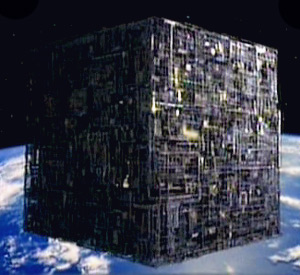
\includegraphics[width=0.3\linewidth]{Borg_cube_orbits_Earth.jpg}
\caption{Data storage in one cell of a staggered MAC grid. (PLACEHOLDER)}
\label{fig:MACgrid}
\end{figure}

When applied to the entire fluid, the advection equation enforces the conservation of energy (the fluid mass undergoes no net acceleration without the application of a net force). The \texttt{advect()} process applies the velocity field to the quantity $q$ for a time $dt$. This quantity may be velocity itself, pressure, or another quantity relevant to the particular fluid (such as temperature for smoke simulation).

Since in truth the fluid is acted on by the net force of gravity, the body process simply adds $\vec{g}dt$ to the velocity field (all the members of the grid).

The incompressibility of the fluid is enforced by the \texttt{project()} process, by subtracting the correct pressure gradient from the output velocity grid of \texttt{body()} (\ref{eq:proj1}).

\begin{equation}
\vec{u}^{n+1}=\vec{u}_B^n-\Delta t\frac{1}{\rho}\nabla p
\label{eq:proj1}
\end{equation}

In numerical form, this results in a series of n equations, where n is the number of cells in the grid. If $\vec{p}$ is a column vector containing all the pressure unknowns, and $\vec{d}$ is a vector of the corresponding divergence values, the series of equations can be written as

\begin{equation}
Ap=d,
\label{eq:apd}
\end{equation}

where A is a symmetric sparse 3D matrix known as the seven-point Lagrangian matrix. Here, this is solved using the Modified Incomplete Cholesky Conjugate Gradient, Level Zero algorithm (MICCG(0)). This involves using the Preconditioned Conjugate Gradient algorithm (shown in Figure \ref{fig:PCG}),

\begin{figure}[h]
\begin{framed}
\texttt{// "$\cdot$" is the dot product of two vectors; "*" is scalar multiplication}

\texttt{p = 0}

\texttt{r = d}

\texttt{z = applyPreconditioner(r)}

\texttt{s = z}

\texttt{$\sigma$ = z $\cdot$ r}

\texttt{iterations = 0}

\texttt{while (p not within tolerance) and (iterations < maximumIterations)}

\texttt{~~~~z = A $\cdot$ s}

\texttt{~~~~$\alpha$ = $\rho$ / (z $\cdot$ s)}

\texttt{~~~~p = p + $\alpha$ * s}

\texttt{~~~~r = r - $\alpha$ * z}

\texttt{~~~~// if the element of r with the greatest absolute value is within}

\texttt{~~~~// tolerance, take current p as the solution}

\texttt{~~~~if (max(|r|) $\leq$ tol) return p}

\texttt{~~~~$\sigma_{new}$ = z $\cdot$ r}

\texttt{~~~~$\beta$ = $\sigma_{new}$ / $\rho$}

\texttt{~~~~}
\end{framed}
\centering
\vspace*{-3mm}\caption{kaejbvksad}
\label{fig:PCG}
\end{figure}

with the \texttt{applyPreconditioner()} function

\begin{figure}[h]
\begin{framed}
\texttt{}

\texttt{}

\texttt{}
\end{framed}
\centering
\vspace*{-3mm}\caption{kaejbvksad}
\label{fig:precond}
\end{figure}

Seven Point Lagrangian Matrix

MIC(0)

preconditioner

Different types of fluids require specific considerations. For smoke, the body force is replaced with a temperature-dependent buoyancy force. Using the Boussinesq approximation of constant pressure, and assuming a linear dependence on only the temperature and smoke concentration  (\ref{eq:fBuoy}
\end{document}
